\documentclass[12pt]{article}
\usepackage[utf8]{inputenc}
\usepackage{mathtools} % also loads amsmath
\usepackage{amsmath,amsthm,amsfonts,amssymb}
\usepackage{tikz}
% \usepackage{subfig}
\usepackage[english]{babel}
\usepackage{capt-of}
\usepackage{tabularray}
\usepackage{caption}
\usepackage{subcaption}
% \usepackage{subcaption}
% \captionsetup{compatibility=false}
\usepackage{graphicx}
\newtheorem{theorem}{Theorem}
\usetikzlibrary{calc}
\usetikzlibrary{shapes}
\usepackage{hyperref}
%might be unnecessary
\usepackage{doi}

%bibliography CMDS

%\usepackage{cite}
%\usepackage[style=alphabetic]{biblatex}
%\bibliographystyle{plain}

%\usepackage[style=alphabetic]{biblatex}

% \usepackage[backend=biber,style=alphabetic]{biblatex}
\usepackage[backend=biber,style=numeric]{biblatex}
% \usepackage[backend=biber,style=abbrv]{biblatex}
% \usepackage[backend=biber,style=alpha]{biblatex}
%\usepackage[backend=bibtex,style=alphabetic]{biblatex}
\addbibresource{./bibb.bib}

%%% With amsthm package, creates environments for nicely formatted,
%%% labeled, and numbered propositions, etc.
\theoremstyle{plain}

\newtheorem{thm}{Theorem}[section]
\newtheorem{lemma}[thm]{Lemma}
\newtheorem{prop}[thm]{Proposition}
\newtheorem{conj}[thm]{Conjecture}
\newtheorem{cor}[thm]{Corollary}
\newtheorem{claim}[thm]{Claim}
\newtheorem{fact}[thm]{Fact}
\newtheorem{constraint}[thm]{Constraint}
\newtheorem{condition}[thm]{Condition}

\theoremstyle{definition}
\newtheorem{eg}[thm]{Example}
% \newtheorem{defn}[thm]{Definition}
\newtheorem{definition}{Definition}[section]
\newtheorem{rem}[thm]{Remark}
\newtheorem{observ}[thm]{Observation}
\newtheorem{open}[thm]{Open Problem}
\newtheorem{prob.}[thm]{Problem}
\newtheorem{quest}[thm]{Question}

% I used these for making definitions and theorems, not what is above
\theoremstyle{remark}
\newtheorem{remark}[thm]{Remark}
\newtheorem{note}[thm]{Note}

\theoremstyle{definition}
% \newtheorem{definition}{Definition}[section]
\newtheorem{exmp}{Example}[section]

%custom commands

% blank cell
\newcommand{\cell}[4]{ \draw[thick] ( #1 , #2 ) rectangle ( #3 , #4 );}

% invisible cell for spacing
\newcommand{\spacecell}[4]{ \draw[thick, color=white] ( #1 , #2 ) rectangle ( #3 , #4 );}

% open cell 
\newcommand{\cellopen}[4]{ \draw[thick] ( #1 , #2 ) rectangle ( #3 , #4 ); \node[shape=circle,draw=red,fill=red, inner sep=0pt,minimum size=3pt] (A) at ( #1 * 0.5 + #3 * 0.5 , #2 * 0.5 + #4 * 0.5 ){};}

\newcommand{\cellA}[4]{ \draw[thick] ( #1 , #2 ) rectangle ( #3 , #4 ); \draw[red, thick, densely dotted] (#3 * 0.5 + #1 * 0.5 , #2) -- (#1, #4 * 0.5 + #2 * 0.5);}
\newcommand{\cellB}[4]{ \draw[thick] ( #1 , #2 ) rectangle ( #3 , #4 ); \draw[red, thick, densely dotted] (#3 * 0.5 + #1 * 0.5 , #2) -- (#3, #4 * 0.5 + #2 * 0.5);}
\newcommand{\cellC}[4]{ \draw[thick] ( #1 , #2 ) rectangle ( #3 , #4 ); \draw[red, thick, densely dotted] (#3 * 0.5 + #1 * 0.5 , #4) -- (#3, #4 * 0.5 + #2 * 0.5);}
\newcommand{\cellD}[4]{ \draw[thick] ( #1 , #2 ) rectangle ( #3 , #4 ); \draw[red, thick, densely dotted] (#3 * 0.5 + #1 * 0.5 , #4) -- (#1, #4 * 0.5 + #2 * 0.5);}
\newcommand{\cellE}[4]{ \draw[thick] ( #1 , #2 ) rectangle ( #3 , #4 ); \draw[red, thick, densely dotted] (#3, #4 * 0.5 + #2 * 0.5) -- (#1, #4 * 0.5 + #2 * 0.5);}
\newcommand{\cellF}[4]{ \draw[thick] ( #1 , #2 ) rectangle ( #3 , #4 ); \draw[red, thick, densely dotted] (#3 * 0.5 + #1 * 0.5 , #2) -- (#3 * 0.5 + #1 * 0.5 , #4);}

\newcommand{\cellAf}[4]{\filldraw[gray!40] ( #1 , #2 ) rectangle ( #3 , #4 ); \draw[thick] ( #1 , #2 ) rectangle ( #3 , #4 ); \draw[red, thick, densely dotted] (#3 * 0.5 + #1 * 0.5 , #2) -- (#1, #4 * 0.5 + #2 * 0.5);}
\newcommand{\cellBf}[4]{\filldraw[gray!40] ( #1 , #2 ) rectangle ( #3 , #4 ); \draw[thick] ( #1 , #2 ) rectangle ( #3 , #4 ); \draw[red, thick, densely dotted] (#3 * 0.5 + #1 * 0.5 , #2) -- (#3, #4 * 0.5 + #2 * 0.5);}
\newcommand{\cellCf}[4]{\filldraw[gray!40] ( #1 , #2 ) rectangle ( #3 , #4 ); \draw[thick] ( #1 , #2 ) rectangle ( #3 , #4 ); \draw[red, thick, densely dotted] (#3 * 0.5 + #1 * 0.5 , #4) -- (#3, #4 * 0.5 + #2 * 0.5);}
\newcommand{\cellDf}[4]{\filldraw[gray!40] ( #1 , #2 ) rectangle ( #3 , #4 ); \draw[thick] ( #1 , #2 ) rectangle ( #3 , #4 ); \draw[red, thick, densely dotted] (#3 * 0.5 + #1 * 0.5 , #4) -- (#1, #4 * 0.5 + #2 * 0.5);}
\newcommand{\cellEf}[4]{\filldraw[gray!40] ( #1 , #2 ) rectangle ( #3 , #4 ); \draw[thick] ( #1 , #2 ) rectangle ( #3 , #4 ); \draw[red, thick, densely dotted] (#3, #4 * 0.5 + #2 * 0.5) -- (#1, #4 * 0.5 + #2 * 0.5);}
\newcommand{\cellFf}[4]{\filldraw[gray!40] ( #1 , #2 ) rectangle ( #3 , #4 ); \draw[thick] ( #1 , #2 ) rectangle ( #3 , #4 ); \draw[red, thick, densely dotted] (#3 * 0.5 + #1 * 0.5 , #2) -- (#3 * 0.5 + #1 * 0.5 , #4);}


% \newcommand{\cellA}[4]{\draw[red, thick, densely dotted] ( #1 + 0.5 , #2 ) arc(0:90:{0.5}); \draw[thick] ( #1 , #2 ) rectangle ( #3 , #4 );}
% \newcommand{\cellB}[4]{\draw[red, thick, densely dotted] ( #1 + 1 , #2 + 0.5 ) arc(90:180:{0.5}); \draw[thick] ( #1 , #2 ) rectangle ( #3 , #4 );}
% \newcommand{\cellC}[4]{\draw[red, thick, densely dotted] ( #1 + 0.5, #2 + 1 ) arc(180:270:{0.5}); \draw[thick] ( #1 , #2 ) rectangle ( #3 , #4 );}
% \newcommand{\cellD}[4]{\draw[red, thick, densely dotted] ( #1 , #2 + 0.5 ) arc(-90:0:{0.5}); \draw[thick] ( #1 , #2 ) rectangle ( #3 , #4 );}
% \newcommand{\cellE}[4]{\draw[red, thick, densely dotted] (#3, #4 * 0.5 + #2 * 0.5) -- (#1, #4 * 0.5 + #2 * 0.5); \draw[thick] ( #1 , #2 ) rectangle ( #3 , #4 );}
% \newcommand{\cellF}[4]{\draw[red, thick, densely dotted] (#3 * 0.5 + #1 * 0.5 , #2) -- (#3 * 0.5 + #1 * 0.5 , #4); \draw[thick] ( #1 , #2 ) rectangle ( #3 , #4 );}
% \newcommand{\cellG}[4]{\draw[red, thick, densely dotted] ( #1 + 0.5 , #2 ) arc(0:90:{0.5}); \draw[red, thick, densely dotted] ( #1 + 0.5, #2 + 1 ) arc(180:270:{0.5}); \draw[thick] ( #1 , #2 ) rectangle ( #3 , #4 );}
% \newcommand{\cellH}[4]{\draw[red, thick, densely dotted] ( #1 , #2 + 0.5 ) arc(-90:0:{0.5}); \draw[red, thick, densely dotted] ( #1 + 1 , #2 + 0.5 ) arc(90:180:{0.5}); \draw[thick] ( #1 , #2 ) rectangle ( #3 , #4 );}
% \newcommand{\cellI}[4]{\draw[red, thick, densely dotted] (#3 * 0.5 + #1 * 0.5 , #2) -- (#3 * 0.5 + #1 * 0.5 , #4); \node[shape=circle,draw=none,fill=white, inner sep=3pt,minimum size=5pt] (A) at ( #1 + 0.5 , #2 + 0.5 ) {}; \draw[red, thick, densely dotted] (#3, #4 * 0.5 + #2 * 0.5) -- (#1, #4 * 0.5 + #2 * 0.5); \draw[thick] ( #1 , #2 ) rectangle ( #3 , #4 );}
% \newcommand{\cellJ}[4]{\draw[red, thick, densely dotted] (#3, #4 * 0.5 + #2 * 0.5) -- (#1, #4 * 0.5 + #2 * 0.5); \node[shape=circle,draw=none,fill=white, inner sep=3pt,minimum size=5pt] (A) at ( #1 + 0.5 , #2 + 0.5 ) {}; \draw[thick] ( #1 , #2 ) rectangle ( #3 , #4 ); \draw[red, thick, densely dotted] (#3 * 0.5 + #1 * 0.5 , #2) -- (#3 * 0.5 + #1 * 0.5 , #4);}

% \newcommand{\cellAf}[4]{\filldraw[gray!40] ( #1 , #2 ) rectangle ( #3 , #4 ); \draw[red, thick, densely dotted] ( #1 + 0.5 , #2 ) arc(0:90:{0.5}); \draw[thick] ( #1 , #2 ) rectangle ( #3 , #4 );}
% \newcommand{\cellBf}[4]{\filldraw[gray!40] ( #1 , #2 ) rectangle ( #3 , #4 ); \draw[red, thick, densely dotted] ( #1 + 1 , #2 + 0.5 ) arc(90:180:{0.5}); \draw[thick] ( #1 , #2 ) rectangle ( #3 , #4 );}
% \newcommand{\cellCf}[4]{\filldraw[gray!40] ( #1 , #2 ) rectangle ( #3 , #4 ); \draw[red, thick, densely dotted] ( #1 + 0.5, #2 + 1 ) arc(180:270:{0.5}); \draw[thick] ( #1 , #2 ) rectangle ( #3 , #4 );}
% \newcommand{\cellDf}[4]{\filldraw[gray!40] ( #1 , #2 ) rectangle ( #3 , #4 ); \draw[red, thick, densely dotted] ( #1 , #2 + 0.5 ) arc(-90:0:{0.5}); \draw[thick] ( #1 , #2 ) rectangle ( #3 , #4 );}
% \newcommand{\cellEf}[4]{\filldraw[gray!40] ( #1 , #2 ) rectangle ( #3 , #4 ); \draw[red, thick, densely dotted] (#3, #4 * 0.5 + #2 * 0.5) -- (#1, #4 * 0.5 + #2 * 0.5); \draw[thick] ( #1 , #2 ) rectangle ( #3 , #4 );}
% \newcommand{\cellFf}[4]{\filldraw[gray!40] ( #1 , #2 ) rectangle ( #3 , #4 ); \draw[red, thick, densely dotted] (#3 * 0.5 + #1 * 0.5 , #2) -- (#3 * 0.5 + #1 * 0.5 , #4); \draw[thick] ( #1 , #2 ) rectangle ( #3 , #4 );}
% \newcommand{\cellGf}[4]{\filldraw[gray!40] ( #1 , #2 ) rectangle ( #3 , #4 ); \draw[red, thick, densely dotted] ( #1 + 0.5 , #2 ) arc(0:90:{0.5}); \draw[red, thick, densely dotted] ( #1 + 0.5, #2 + 1 ) arc(180:270:{0.5}); \draw[thick] ( #1 , #2 ) rectangle ( #3 , #4 );}
% \newcommand{\cellHf}[4]{\filldraw[gray!40] ( #1 , #2 ) rectangle ( #3 , #4 ); \draw[red, thick, densely dotted] ( #1 , #2 + 0.5 ) arc(-90:0:{0.5}); \draw[red, thick, densely dotted] ( #1 + 1 , #2 + 0.5 ) arc(90:180:{0.5}); \draw[thick] ( #1 , #2 ) rectangle ( #3 , #4 );}
% \newcommand{\cellIf}[4]{\filldraw[gray!40] ( #1 , #2 ) rectangle ( #3 , #4 ); \draw[red, thick, densely dotted] (#3 * 0.5 + #1 * 0.5 , #2) -- (#3 * 0.5 + #1 * 0.5 , #4); \node[shape=circle,draw=none,fill=gray!40, inner sep=3pt,minimum size=5pt] (A) at ( #1 + 0.5 , #2 + 0.5 ) {}; \draw[red, thick, densely dotted] (#3, #4 * 0.5 + #2 * 0.5) -- (#1, #4 * 0.5 + #2 * 0.5); \draw[thick] ( #1 , #2 ) rectangle ( #3 , #4 );}
% \newcommand{\cellJf}[4]{\filldraw[gray!40] ( #1 , #2 ) rectangle ( #3 , #4 ); \draw[red, thick, densely dotted] (#3, #4 * 0.5 + #2 * 0.5) -- (#1, #4 * 0.5 + #2 * 0.5); \node[shape=circle,draw=none,fill=gray!40, inner sep=3pt,minimum size=5pt] (A) at ( #1 + 0.5 , #2 + 0.5 ) {}; \draw[thick] ( #1 , #2 ) rectangle ( #3 , #4 ); \draw[red, thick, densely dotted] (#3 * 0.5 + #1 * 0.5 , #2) -- (#3 * 0.5 + #1 * 0.5 , #4);}


\newcommand{\lablnode}[3]{\node[shape=circle,draw=none,fill=none, inner sep=0pt,minimum size=0pt] (A) at ( #1 , #2 ) {#3};}
\newcommand{\lablvertex}[3]{\node[shape=circle,draw=none,fill=white, inner sep=2pt,minimum size=5pt] (A) at ( #1 , #2 ) {#3};}

\usepackage[margin=1in]{geometry}
\date{}
%doc info
\author{
    \textbf{Jack Hanke}\\
    Northwestern University
    \and
    \textbf{Michael Maltenfort}\\
    Northwestern University
    % \and
    % \textbf{Richard Schank}\\
    }
\title{\textbf{Enumeration of Messy Polygon Mosaics}}
% \date{\today}

\begin{document}
\maketitle

\begin{center}

\begin{abstract}
Hong and Oh introduced a model for multiple ring polymers in physics in which an $m \times n$ matrix is constructed from a selection of $7$ distinct tiles. These matrices are called \textit{mosaics}. The authors provide bounds on a subset of these mosaics that have the property of being suitably connected. These mosaics are called \textit{polygon mosaics} because the tiles in a suitably connected mosaic form polygons. We introduce and enumerate mosaics with the related property of containing at least one polygon, which we call messy polygon mosaics.
\end{abstract}

\end{center}

\section{Introduction}

Hong and Oh \cite{Hong2018} introduced a model for multiple ring polymers in which an $m \times n$ matrix is constructed using $7$ distinct symbols callet \textit{tiles}. These tiles, diagrammed in Figure \ref{fig:tile set}, are composed of unit squares with dotted lines connecting $2$ sides at their midpoint, as well as the ``blank" tile $T_0$.

\begin{figure}[h!]
\begin{center}
    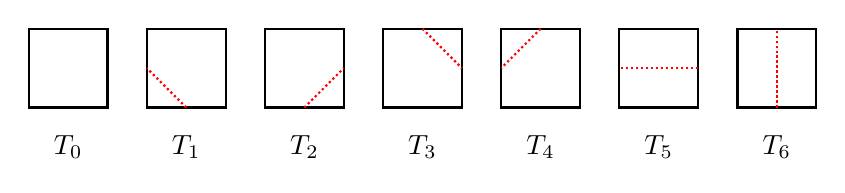
\begin{tikzpicture}
        \cell{0}{0}{1}{1}
        \( \lablnode{0.5}{-0.5}{$T_0$} \) 
        \cellA{1.5}{0}{2.5}{1}
        \( \lablnode{2}{-0.5}{$T_1$} \) 
        \cellB{3}{0}{4}{1}
        \( \lablnode{3.5}{-0.5}{$T_2$} \) 
        \cellC{4.5}{0}{5.5}{1}
        \( \lablnode{5}{-0.5}{$T_3$} \) 
        \cellD{6}{0}{7}{1}
        \( \lablnode{6.5}{-0.5}{$T_4$} \) 
        \cellE{7.5}{0}{8.5}{1}
        \( \lablnode{8}{-0.5}{$T_5$} \) 
        \cellF{9}{0}{10}{1}
        \( \lablnode{9.5}{-0.5}{$T_6$} \) 
        % \cellG{10.5}{0}{11.5}{1}
        % \( \lablnode{11}{-0.5}{$T_7$} \) 
        % \cellH{12}{0}{13}{1}
        % \( \lablnode{12.5}{-0.5}{$T_8$} \) 
        % \cellI{13.5}{0}{14.5}{1}
        % \( \lablnode{14}{-0.5}{$T_{9}$} \) 
        % \cellJ{15}{0}{16}{1}
        % \( \lablnode{15.5}{-0.5}{$T_{10}$} \) 
    \end{tikzpicture}
\end{center}
\caption{The tile set $\mathbb{T}$}
\label{fig:tile set}
\end{figure}

We denote the set of tiles $\mathbb{T}=\{T_0, \dots, T_{6}\}$. An $(m,n)$ \textit{mosaic} is an $m \times n$ matrix made up of elements from $\mathbb{T}$. Figure \ref{fig:example mosaic} shows a $(5,7)$ mosaic. We denote the set of all $(m,n)$ mosaics as $\mathbb{M}^{(m,n)}$. As there are $7$ elements in $\mathbb{T}$, there are $7^{mn}$ mosaics in $\mathbb{M}^{(m,n)}$. 
% A \textit{mosaic system} is then a subset of $\mathbb{M}^{(m,n)}$ with some property. 

\begin{figure}[h!]
    \begin{center}
    \begin{subfigure}{0.4\textwidth}
        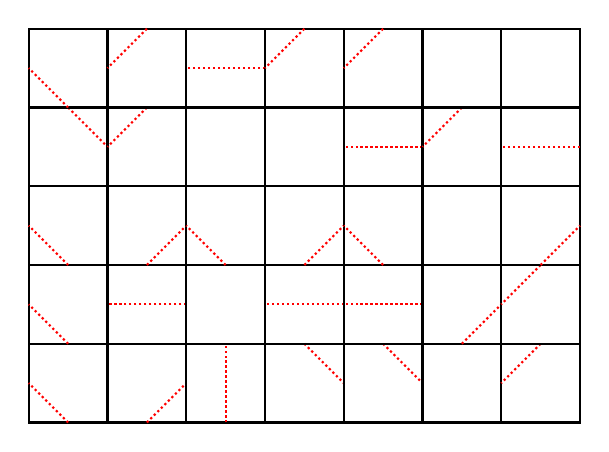
\begin{tikzpicture}
        % row1
        \cellA{0}{0}{1}{1}
        \cellB{1}{0}{2}{1}
        \cellF{2}{0}{3}{1}
        \cellC{3}{0}{4}{1}
        \cellC{4}{0}{5}{1}
        \cell{5}{0}{6}{1}
        \cellD{6}{0}{7}{1}
        % row2
        \cellA{0}{1}{1}{2}
        \cellE{1}{1}{2}{2}
        \cell{2}{1}{3}{2}
        \cellE{3}{1}{4}{2}
        \cellE{4}{1}{5}{2}
        \cellB{5}{1}{6}{2}
        \cellD{6}{1}{7}{2}
        % row3
        \cellA{0}{2}{1}{3}
        \cellB{1}{2}{2}{3}
        \cellA{2}{2}{3}{3}
        \cellB{3}{2}{4}{3}
        \cellA{4}{2}{5}{3}
        \cell{5}{2}{6}{3}
        \cellB{6}{2}{7}{3}
        % row4
        \cellC{0}{3}{1}{4}
        \cellD{1}{3}{2}{4}
        \cell{2}{3}{3}{4}
        \cell{3}{3}{4}{4}
        \cellE{4}{3}{5}{4}
        \cellD{5}{3}{6}{4}
        \cellE{6}{3}{7}{4}
        % row5
        \cellA{0}{4}{1}{5}
        \cellD{1}{4}{2}{5}
        \cellE{2}{4}{3}{5}
        \cellD{3}{4}{4}{5}
        \cellD{4}{4}{5}{5}
        \cell{5}{4}{6}{5}
        \cell{6}{4}{7}{5}
        \end{tikzpicture}
    \caption{A mosaic}
    \label{fig:example mosaic}
    \end{subfigure}
% \hfill
\hspace{0.05\textwidth}
\begin{subfigure}{0.4\textwidth}
    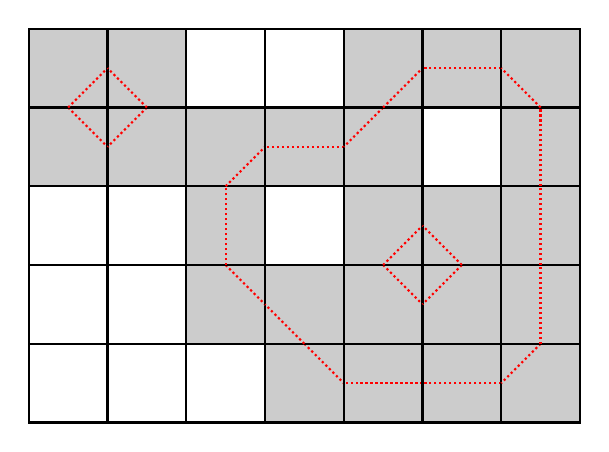
\begin{tikzpicture}
        % row1
        \cell{0}{0}{1}{1}
        \cell{1}{0}{2}{1}
        \cell{2}{0}{3}{1}
        \cellCf{3}{0}{4}{1}
        \cellEf{4}{0}{5}{1}
        \cellEf{5}{0}{6}{1}
        \cellDf{6}{0}{7}{1}
        % row2
        \cell{0}{1}{1}{2}
        \cell{1}{1}{2}{2}
        \cellCf{2}{1}{3}{2}
        \cellAf{3}{1}{4}{2}
        \cellCf{4}{1}{5}{2}
        \cellDf{5}{1}{6}{2}
        \cellFf{6}{1}{7}{2}
        % row3
        \cell{0}{2}{1}{3}
        \cell{1}{2}{2}{3}
        \cellFf{2}{2}{3}{3}
        \cell{3}{2}{4}{3}
        \cellBf{4}{2}{5}{3}
        \cellAf{5}{2}{6}{3}
        \cellFf{6}{2}{7}{3}
        % row4
        \cellCf{0}{3}{1}{4}
        \cellDf{1}{3}{2}{4}
        \cellBf{2}{3}{3}{4}
        \cellEf{3}{3}{4}{4}
        \cellDf{4}{3}{5}{4}
        \cell{5}{3}{6}{4}
        \cellFf{6}{3}{7}{4}
        % row5
        \cellBf{0}{4}{1}{5}
        \cellAf{1}{4}{2}{5}
        \cell{2}{4}{3}{5}
        \cell{3}{4}{4}{5}
        \cellBf{4}{4}{5}{5}
        \cellEf{5}{4}{6}{5}
        \cellAf{6}{4}{7}{5}
    \end{tikzpicture}
    \caption{A polygon mosaic}
    \label{fig:example polygon mosaic}
\end{subfigure}

\end{center}
\caption{Examples of mosaics of size $(5,7)$ made of tiles in $\mathbb{T}$}
\label{fig:example mosaics}
\end{figure}

The authors in \cite{Hong2018} were interested in mosaics with the property of being \textit{suitably connected}, which is defined as follows. Consider an edge shared between two tiles in Figure \ref{fig:example mosaic}. The edge has either $0$, $1$, or $2$ dotted lines drawn from its midpoint. Also note that the outer edges of the tiles on the boundary of the matrix are not shared by another tile. Therefore these edges only have $0$ or $1$ dotted lines drawn from their midpoint. A mosaic is suitably connected if all edges have $0$ or $2$ dotted lines drawn from their midpoint. The authors call mosaics that are suitably connected and that contain at least one tile in $\mathbb{T}\setminus T_0$ \textit{polygon mosaics} because the dotted lines form \textit{polygons}\footnote{Polygons are more commonly refered to as ``self-avoiding polygons" in the literature to highlight their connection with self-avoiding walks.}. Following \cite{Hong2018}, when we use the term polygon in this work, we specifically refer to the set of tiles for which the dotted lines form a polygon when part of a mosaic.

\begin{exmp}
Figure \ref{fig:example polygon mosaic} shows a polygon $(5,7)$ mosaic that contains $3$ polygons, with the tiles that make up the polygons shaded in gray. Note that a mosaic can contain polygons that surround other polygons, such as in Figure \ref{fig:example polygon mosaic}. 

\begin{figure}[h!]
\begin{center}
    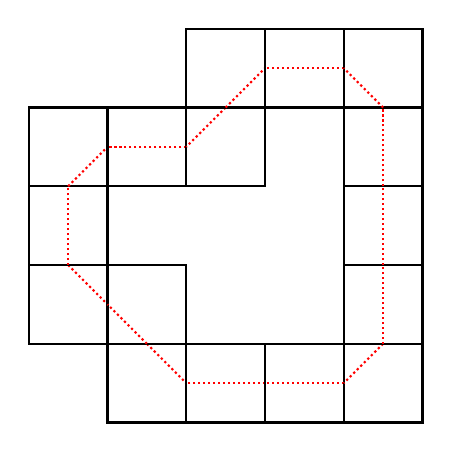
\begin{tikzpicture}
        % row1
        \cellC{3}{0}{4}{1}
        \cellE{4}{0}{5}{1}
        \cellE{5}{0}{6}{1}
        \cellD{6}{0}{7}{1}
        % row2
        \cellC{2}{1}{3}{2}
        \cellA{3}{1}{4}{2}
        \cellF{6}{1}{7}{2}
        % row3
        \cellF{2}{2}{3}{3}
        \cellF{6}{2}{7}{3}
        % row4
        \cellB{2}{3}{3}{4}
        \cellE{3}{3}{4}{4}
        \cellD{4}{3}{5}{4}
        \cellF{6}{3}{7}{4}
        % row5
        \cellB{4}{4}{5}{5}
        \cellE{5}{4}{6}{5}
        \cellA{6}{4}{7}{5}
    \end{tikzpicture}
\caption{A polygon in Figure \ref{fig:example polygon mosaic}}
\label{fig: example polygon}
\end{center}
\end{figure}
\end{exmp}

Using the notation conventions in \cite{Oh2014}, we denote the subset of $(m,n)$ mosaics that are polygon mosaics as $\mathbb{P}^{(m,n)}$.

\begin{thm}[\cite{Hong2018}]
\label{thm:Hong2018}
The number of polygon $(m,n)$ mosaics $|\mathbb{P}^{(m,n)}|$ for $m,n \geq 3$ is bounded by
$$2^{m+n-3}\left(\frac{17}{10}\right)^{(m-2)(n-2)} \leq |\mathbb{P}^{(m,n)}| \leq 2^{m+n-3}\left(\frac{31}{16}\right)^{(m-2)(n-2)}.$$
\end{thm}

The array of values of $|\mathbb{P}^{(m,n)}|+1$ is sequence A181245 on the OEIS \cite[OEIS]{oeis}.

In related work, Lomonaco and Kauffman \cite{Lomonaco08} introduced mosaics constructed from a tile set of $11$ distinct tiles, of which $\mathbb{T}$ is a subset. The authors call mosaics constructed from this tile set that are suitably connected \textit{knot mosaics}. Oh et al. \cite{Oh2014} enumerated the number of knot mosaics.

\begin{thm}[\cite{Oh2014}]
\label{thm:Oh2014}
The number of knot mosaics of size $(m,n)$ for $m,n \geq 2$ is $2 \left\| (X_{m-2}+O_{m-2})^{n-2} \right\|$, where $X_0 = O_0 = \begin{bmatrix} 1 \\ \end{bmatrix}$ and $X_{m-2}$ and $O_{m-2}$ are $2^{m-2} \times 2^{m-2}$ matrices defined as

$$ X_{k+1} = \begin{pmatrix}
    X_k & O_k \\
    O_k & X_k
\end{pmatrix}
\text{ and }
O_{k+1} = \begin{pmatrix}
    O_k & X_k \\
    X_k & 4O_k
\end{pmatrix}, $$

for $k=0,1,\dots,m-3$. Here $\left\| N \right\|$ denotes the sum of elements of matrix $N$.
\end{thm}

Oh and colleagues refer to these matrices $X_k$ and $O_k$ as \textit{state matrices}. The authors utilize this state matrix recursion to bound the growth rate of knot mosaics \cite{Oh2016, Oh2019, Choi2024}, and Oh further adapts the method to solve problems in monomer and dimer tilings \cite{Oh2018Aztec, Oh2019tiling}. An unexamined direction in this research program is modifying the suitably connected property. This motivates us to introduce \textit{messy polygon mosaics} using the tiles set $\mathbb{T}$ from \cite{Hong2018}, and enumerate them with state matrices as in \cite{Oh2014}.

\section{Messy Polygon Mosaics}\label{section:messy mosaics}

\begin{definition}
A \textit{messy polygon mosaic} is a mosaic that contains at least one polygon. 
\end{definition}

Figure \ref{fig:messy mosaic example} shows two examples of messy polygon $(5,7)$ mosaics, both of which contain $3$ polygons. In both examples, we shade the tiles that make up each polygon in gray.

\begin{figure}[h!]
    \begin{center}

\begin{subfigure}{0.4\textwidth}
    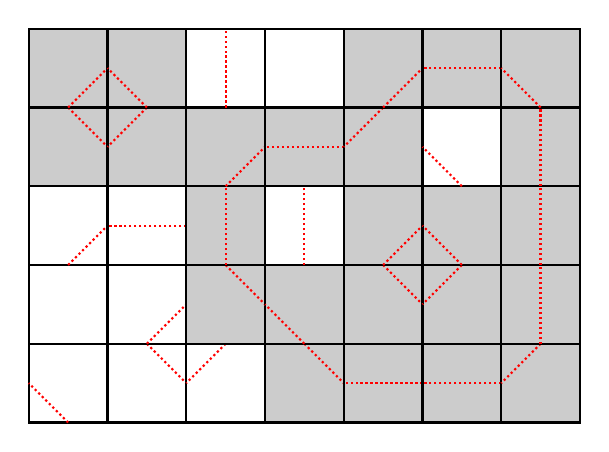
\begin{tikzpicture}
       % row1
        \cellA{0}{0}{1}{1}
        \cellC{1}{0}{2}{1}
        \cellD{2}{0}{3}{1}
        \cellCf{3}{0}{4}{1}
        \cellEf{4}{0}{5}{1}
        \cellEf{5}{0}{6}{1}
        \cellDf{6}{0}{7}{1}
        % row2
        \cell{0}{1}{1}{2}
        \cellB{1}{1}{2}{2}
        \cellCf{2}{1}{3}{2}
        \cellAf{3}{1}{4}{2}
        \cellCf{4}{1}{5}{2}
        \cellDf{5}{1}{6}{2}
        \cellFf{6}{1}{7}{2}
        % row3
        \cellB{0}{2}{1}{3}
        \cellE{1}{2}{2}{3}
        \cellFf{2}{2}{3}{3}
        \cellF{3}{2}{4}{3}
        \cellBf{4}{2}{5}{3}
        \cellAf{5}{2}{6}{3}
        \cellFf{6}{2}{7}{3}
        % row4
        \cellCf{0}{3}{1}{4}
        \cellDf{1}{3}{2}{4}
        \cellBf{2}{3}{3}{4}
        \cellEf{3}{3}{4}{4}
        \cellDf{4}{3}{5}{4}
        \cellA{5}{3}{6}{4}
        \cellFf{6}{3}{7}{4}
        % row5
        \cellBf{0}{4}{1}{5}
        \cellAf{1}{4}{2}{5}
        \cellF{2}{4}{3}{5}
        \cell{3}{4}{4}{5}
        \cellBf{4}{4}{5}{5}
        \cellEf{5}{4}{6}{5}
        \cellAf{6}{4}{7}{5}
    \end{tikzpicture}
\end{subfigure}
% \hfill
\hspace{0.05\textwidth}
\begin{subfigure}{0.4\textwidth}
        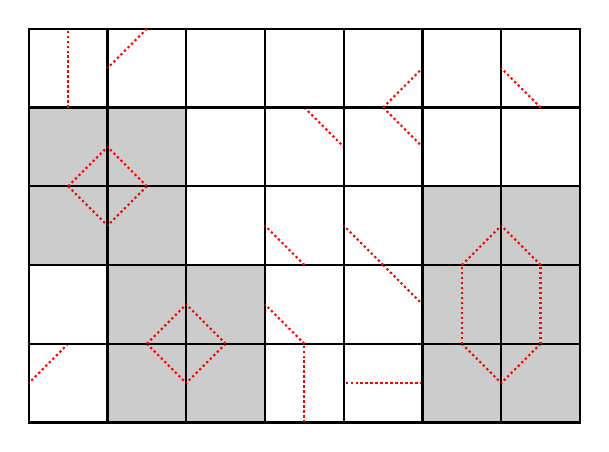
\begin{tikzpicture}
        % row1
        \cellD{0}{0}{1}{1}
        \cellCf{1}{0}{2}{1}
        \cellDf{2}{0}{3}{1}
        \cellF{3}{0}{4}{1}
        \cellE{4}{0}{5}{1}
        \cellCf{5}{0}{6}{1}
        \cellDf{6}{0}{7}{1}
        % row2
        \cell{0}{1}{1}{2}
        \cellBf{1}{1}{2}{2}
        \cellAf{2}{1}{3}{2}
        \cellA{3}{1}{4}{2}
        \cellC{4}{1}{5}{2}
        \cellFf{5}{1}{6}{2}
        \cellFf{6}{1}{7}{2}
        % row3
        \cellCf{0}{2}{1}{3}
        \cellDf{1}{2}{2}{3}
        \cell{2}{2}{3}{3}
        \cellA{3}{2}{4}{3}
        \cellA{4}{2}{5}{3}
        \cellBf{5}{2}{6}{3}
        \cellAf{6}{2}{7}{3}
        % row4
        \cellBf{0}{3}{1}{4}
        \cellAf{1}{3}{2}{4}
        \cell{2}{3}{3}{4}
        \cellC{3}{3}{4}{4}
        \cellC{4}{3}{5}{4}
        \cell{5}{3}{6}{4}
        \cell{6}{3}{7}{4}
        % row5
        \cellF{0}{4}{1}{5}
        \cellD{1}{4}{2}{5}
        \cell{2}{4}{3}{5}
        \cell{3}{4}{4}{5}
        \cellB{4}{4}{5}{5}
        \cell{5}{4}{6}{5}
        \cellA{6}{4}{7}{5}
    \end{tikzpicture}
\end{subfigure}

\end{center}
\caption{Examples of $(5,7$) messy polygon mosaics}
\label{fig:messy mosaic example}
\end{figure}

The main goal of this paper is to enumerate messy polygon mosaics, but it turns out to be simpler to enumerate the number of mosaics that \textit{do not} contain a polygon. Therefore, let $\mathbb{S}^{(m,n)}$ be the subset of $(m,n)$ mosaics that do not contain a polygon. Clearly the number of messy polygon $(m,n)$ mosaics is then $7^{mn} - \left|\mathbb{S}^{(m,n)}\right|$.

From the fact that the smallest polygon is made of $4$ tiles, shown in Figure \ref{fig:smallest polygon}, we can conclude that $\left|\mathbb{S}^{(n,1)}\right|=7^n$, and $\left|\mathbb{S}^{(2,2)}\right| = 7^4 - 1$. For $n,m \geq 2$, we first define the state matrices for messy polygon mosaics.

\begin{figure}[h!]
    \begin{center}
    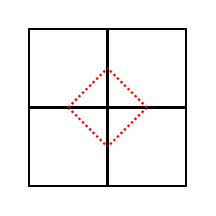
\begin{tikzpicture}
        % row1
        \cellC{0}{0}{1}{1}
        \cellD{1}{0}{2}{1}
        % row2
        \cellB{0}{1}{1}{2}
        \cellA{1}{1}{2}{2}
    \end{tikzpicture}
    \end{center}
    \caption{The smallest polygon}
    \label{fig:smallest polygon}
\end{figure}

\begin{definition}

For integers $k \geq 1$ let $A_k, B_k, C_k, D_k$ be $2^{k-1} \times 2^{k-1}$ matrices with integer entries, where $A_{1}=\begin{pmatrix}7\end{pmatrix}, B_{1}=\begin{pmatrix}-1\end{pmatrix}, C_{1}=\begin{pmatrix}1\end{pmatrix}, D_{1}=\begin{pmatrix}1\end{pmatrix}$ and

\begin{eqnarray*}
A_{k+1} = \begin{pmatrix} 7A_{k} & B_{k} \\ C_{k} & D_{k} \end{pmatrix} & B_{k+1} = \begin{pmatrix} -A_{k} & B_{k} \\ 0C_{k} & D_{k} \end{pmatrix} \\
C_{k+1} = \begin{pmatrix} A_{k} & 0B_{k} \\ C_{k} & D_{k} \end{pmatrix} & D_{k+1} = \begin{pmatrix} A_{k} & -B_{k} \\ C_{k} & 7D_{k} \end{pmatrix}.
\end{eqnarray*}

\end{definition}

Our main result is Theorem \ref{thm: messy mosaics}.

\begin{thm}
\label{thm: messy mosaics}
The number of $(m,n)$ mosaics that do not contain a polygon $\left|\mathbb{S}^{(m,n)}\right|$ is the $(0,0)$ entry of $A_{n}^m$.
\end{thm}

\section{Preliminaries}

% TODO essentially change all this lol \begingroup $\setlength\arraycolsep{1pt}\arrayrowsep{1pt}\begin{matrix} 1 & 0 \\ 1 & 1 \\ \end{matrix}$\endgroup

We begin by defining a mapping $f$ between a mosaic in $\mathbb{M}^{(m,n)}$ to an $(m,n)$ \textit{binary lattice}. An $(m,n)$ binary lattice is a rectangular lattice of $m+1$ by $n+1$ vertices, with each vertex labeled $0$ or $1$. We also define a \textit{framed} binary lattice to be a binary lattice in which the boundary vertices are labeled $0$. An example of a $(5,7)$ framed binary lattice is shown on the right of Figure \ref{fig:example of f mapping}. Also let $\mathbb{L}^{(m,n)}$ be the set of all $(m,n)$ binary lattices and $\mathbb{F}^{(m,n)}$ be the set of all $(m,n)$ framed binary lattices. We immediately have $\left|\mathbb{L}^{(m,n)}\right| = 2^{(m+1)(n+1)}$, $\left|\mathbb{F}^{(m,n)}\right| = 2^{(m-1)(n-1)}$. 

\begin{definition}

$f: \mathbb{M}^{(m,n)} \to \mathbb{F}^{(m,n)}$ takes a mosaic and labels each vertex with the following rule. If the vertex is surrounded by an even number of polygons (including $0$ polygons), label it $0$. If the vertex is surrounded by an odd number of polygons, label it $1$. Removing the red dotted lines from the tiles gives the framed binary lattice. 
    
\end{definition}

\begin{figure}
\begin{center}
    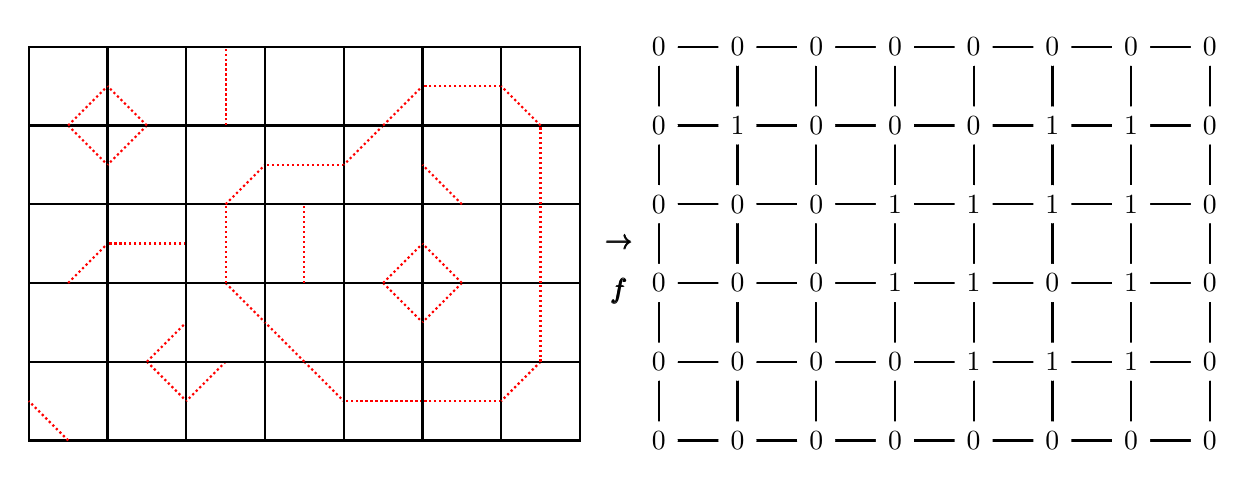
\begin{tikzpicture}
        % row1
        \cellA{0}{0}{1}{1}
        \cellC{1}{0}{2}{1}
        \cellD{2}{0}{3}{1}
        \cellC{3}{0}{4}{1}
        \cellE{4}{0}{5}{1}
        \cellE{5}{0}{6}{1}
        \cellD{6}{0}{7}{1}
        % row2
        \cell{0}{1}{1}{2}
        \cellB{1}{1}{2}{2}
        \cellC{2}{1}{3}{2}
        \cellA{3}{1}{4}{2}
        \cellC{4}{1}{5}{2}
        \cellD{5}{1}{6}{2}
        \cellF{6}{1}{7}{2}
        % row3
        \cellB{0}{2}{1}{3}
        \cellE{1}{2}{2}{3}
        \cellF{2}{2}{3}{3}
        \cellF{3}{2}{4}{3}
        \cellB{4}{2}{5}{3}
        \cellA{5}{2}{6}{3}
        \cellF{6}{2}{7}{3}
        % row4
        \cellC{0}{3}{1}{4}
        \cellD{1}{3}{2}{4}
        \cellB{2}{3}{3}{4}
        \cellE{3}{3}{4}{4}
        \cellD{4}{3}{5}{4}
        \cellA{5}{3}{6}{4}
        \cellF{6}{3}{7}{4}
        % row5
        \cellB{0}{4}{1}{5}
        \cellA{1}{4}{2}{5}
        \cellF{2}{4}{3}{5}
        \cell{3}{4}{4}{5}
        \cellB{4}{4}{5}{5}
        \cellE{5}{4}{6}{5}
        \cellA{6}{4}{7}{5}
        % arrow
        \( \lablnode{7.5}{2.5}{$\pmb{\to}$} \)
        % 
        \( \lablnode{7.5}{1.9}{$\pmb{f}$} \)

        % row1
        \cell{8}{0}{9}{1}
        \cell{9}{0}{10}{1}
        \cell{10}{0}{11}{1}
        \cell{11}{0}{12}{1}
        \cell{12}{0}{13}{1}
        \cell{13}{0}{14}{1}
        \cell{14}{0}{15}{1}
        % row2
        \cell{8}{1}{9}{2}
        \cell{9}{1}{10}{2}
        \cell{10}{1}{11}{2}
        \cell{11}{1}{12}{2}
        \cell{12}{1}{13}{2}
        \cell{13}{1}{14}{2}
        \cell{14}{1}{15}{2}
        % row3
        \cell{8}{2}{9}{3}
        \cell{9}{2}{10}{3}
        \cell{10}{2}{11}{3}
        \cell{11}{2}{12}{3}
        \cell{12}{2}{13}{3}
        \cell{13}{2}{14}{3}
        \cell{14}{2}{15}{3}
        % row4
        \cell{8}{3}{9}{4}
        \cell{9}{3}{10}{4}
        \cell{10}{3}{11}{4}
        \cell{11}{3}{12}{4}
        \cell{12}{3}{13}{4}
        \cell{13}{3}{14}{4}
        \cell{14}{3}{15}{4}
        % row5
        \cell{8}{4}{9}{5}
        \cell{9}{4}{10}{5}
        \cell{10}{4}{11}{5}
        \cell{11}{4}{12}{5}
        \cell{12}{4}{13}{5}
        \cell{13}{4}{14}{5}
        \cell{14}{4}{15}{5}

        % label for row1
        \( \lablvertex{8}{0}{$0$} \)
        \( \lablvertex{9}{0}{$0$} \)
        \( \lablvertex{10}{0}{$0$} \)
        \( \lablvertex{11}{0}{$0$} \)
        \( \lablvertex{12}{0}{$0$} \)
        \( \lablvertex{13}{0}{$0$} \)
        \( \lablvertex{14}{0}{$0$} \)
        \( \lablvertex{15}{0}{$0$} \)
        % label for row1
        \( \lablvertex{8}{1}{$0$} \)
        \( \lablvertex{9}{1}{$0$} \)
        \( \lablvertex{10}{1}{$0$} \)
        \( \lablvertex{11}{1}{$0$} \)
        \( \lablvertex{12}{1}{$1$} \)
        \( \lablvertex{13}{1}{$1$} \)
        \( \lablvertex{14}{1}{$1$} \)
        \( \lablvertex{15}{1}{$0$} \)
        % label for row1
        \( \lablvertex{8}{2}{$0$} \)
        \( \lablvertex{9}{2}{$0$} \)
        \( \lablvertex{10}{2}{$0$} \)
        \( \lablvertex{11}{2}{$1$} \)
        \( \lablvertex{12}{2}{$1$} \)
        \( \lablvertex{13}{2}{$0$} \)
        \( \lablvertex{14}{2}{$1$} \)
        \( \lablvertex{15}{2}{$0$} \)
        % label for row1
        \( \lablvertex{8}{3}{$0$} \)
        \( \lablvertex{9}{3}{$0$} \)
        \( \lablvertex{10}{3}{$0$} \)
        \( \lablvertex{11}{3}{$1$} \)
        \( \lablvertex{12}{3}{$1$} \)
        \( \lablvertex{13}{3}{$1$} \)
        \( \lablvertex{14}{3}{$1$} \)
        \( \lablvertex{15}{3}{$0$} \)
        % label for row1
        \( \lablvertex{8}{4}{$0$} \)
        \( \lablvertex{9}{4}{$1$} \)
        \( \lablvertex{10}{4}{$0$} \)
        \( \lablvertex{11}{4}{$0$} \)
        \( \lablvertex{12}{4}{$0$} \)
        \( \lablvertex{13}{4}{$1$} \)
        \( \lablvertex{14}{4}{$1$} \)
        \( \lablvertex{15}{4}{$0$} \)
        % label for row1
        \( \lablvertex{8}{5}{$0$} \)
        \( \lablvertex{9}{5}{$0$} \)
        \( \lablvertex{10}{5}{$0$} \)
        \( \lablvertex{11}{5}{$0$} \)
        \( \lablvertex{12}{5}{$0$} \)
        \( \lablvertex{13}{5}{$0$} \)
        \( \lablvertex{14}{5}{$0$} \)
        \( \lablvertex{15}{5}{$0$} \)

    \end{tikzpicture}
\end{center}
\caption{$f$ applied to the left mosaic in Figure \ref{fig:messy mosaic example}, resulting in a binary lattice}
\label{fig:example of f mapping}
\end{figure}

Notice that by the definition of $f$, in a binary lattice polygons draw out the boundary between edge-connected vertices with the same label, excluding the vertices that are edge-connected to the boundary $0$'s. For example in Figure \ref{fig:example of f mapping} the three polygons correspond with the boundary of the three edge-connected regions of vertices that are not edge-connected to the boundary $0$'s.

To enumerate $|\mathbb{S}^{(m,n)}|$, it will be useful to consider how $f$ maps individual tiles in $\mathbb{T}$ to individual \textit{cells} in a binary lattice.

\begin{definition}
Let a \textit{cell} be a $(1,1)$ binary lattice.
\end{definition}

\begin{exmp}
\label{exmp: tile to cell}
Applying $f$ to the mosaic in Figure \ref{fig:example of f mapping} results in the top-left tile $T_2$ mapping to the top-left cell diagrammed below.

\begin{center}
    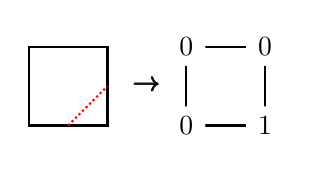
\begin{tikzpicture}
        \cellB{0}{0}{1}{1}
        
        \( \lablnode{1.5}{0.5}{$\pmb{\to}$} \)
        \cell{2}{0}{3}{1}
        
        \( \lablvertex{2}{0}{$0$} \)
        \( \lablvertex{2}{1}{$0$} \)
        \( \lablvertex{3}{0}{$1$} \)
        \( \lablvertex{3}{1}{$0$} \)
    \end{tikzpicture}
\end{center}
\end{exmp}

For convenience, we denote a cell by the $2 \times 2$ matrix of its vertex labels.  For example, we denote the cell in Example \ref{exmp: tile to cell} as $\begin{smallmatrix} 0 & 0 \\ 0 & 1 \end{smallmatrix}$. The set of all unique cells is 
$$\{\begin{smallmatrix} 0 & 0 \\ 0 & 0 \end{smallmatrix}, \begin{smallmatrix} 0 & 0 \\ 0 & 1 \end{smallmatrix}, \begin{smallmatrix} 0 & 0 \\ 1 & 0 \end{smallmatrix}, \begin{smallmatrix} 0 & 0 \\ 1 & 1 \end{smallmatrix},\begin{smallmatrix} 0 & 1 \\ 0 & 0 \end{smallmatrix}, \begin{smallmatrix} 0 & 1 \\ 0 & 1 \end{smallmatrix},\begin{smallmatrix} 0 & 1 \\ 1 & 0 \end{smallmatrix}, \begin{smallmatrix} 0 & 1 \\ 1 & 1 \end{smallmatrix},\begin{smallmatrix} 1 & 0 \\ 0 & 0 \end{smallmatrix}, \begin{smallmatrix} 1 & 0 \\ 0 & 1 \end{smallmatrix},\begin{smallmatrix} 1 & 0 \\ 1 & 0 \end{smallmatrix}, \begin{smallmatrix} 1 & 0 \\ 1 & 1 \end{smallmatrix},\begin{smallmatrix} 1 & 1 \\ 0 & 0 \end{smallmatrix}, \begin{smallmatrix} 1 & 1 \\ 0 & 1 \end{smallmatrix},\begin{smallmatrix} 1 & 1 \\ 1 & 0 \end{smallmatrix}, \begin{smallmatrix} 1 & 1 \\ 1 & 1 \end{smallmatrix}\}.$$

\begin{definition}
    For a given $(m,n)$, let $\ell^*$ be the framed binary lattice made of only $\begin{smallmatrix} 0 & 0 \\ 0 & 0 \end{smallmatrix}$ cells.
    \label{def:all zeros}
\end{definition}

Therefore, as all mosaics that do not contain a polygon map to $\ell^*$ under $f$, we have

\begin{equation}
\label{eq: guiding eq}
\mathbb{S}^{(m,n)} = f^{-1}(\{\ell^*\}),
\end{equation}

and so it suffices to compute $|f^{-1}(\{\ell^*\})|$. 

It would be convenient to compute $f^{-1}(\ell)$ for any binary lattice $\ell$ ``cell-by-cell''. Let $u: \mathbb{L}^{(m,n)} \to \mathbb{N}$  map a binary lattice $\ell$ to the product over all cells in $\ell$ with each term being $$\begin{cases}
        7 & \text{for cells } \begin{smallmatrix} 0 & 0 \\ 0 & 0 \end{smallmatrix}, \begin{smallmatrix} 1 & 1 \\ 1 & 1 \end{smallmatrix}\\
        0 & \text{for cells } \begin{smallmatrix} 0 & 1 \\ 1 & 0 \end{smallmatrix}, \begin{smallmatrix} 1 & 0 \\ 0 & 1 \end{smallmatrix}\\
        1 & \text{otherwise,}
    \end{cases}$$

where these terms come from the number of tiles in $\mathbb{T}$ that can map to a specific cell under $f$. For a given binary lattice $\ell$ that does not contain  $\begin{smallmatrix} 0 & 1 \\ 1 & 0 \end{smallmatrix}$ or $\begin{smallmatrix} 1 & 0 \\ 0 & 1 \end{smallmatrix}$ cells, the function $u(\ell)$ enumerates a set of mosaics of a specific form, in which at each square a tile is either uniquely specified, or can be any tile in $\mathbb{T}$. We can depict this set with a \textit{mosaic diagram}, where we introduce a notational tile with a red dot at the center to indicate that any tile in $\mathbb{T}$ can be in that location (to avoid confusion with the $T_0$ tile). For example, the mosaic diagram for the binary lattice in Figure \ref{fig:example of f mapping} is depicted in Figure \ref{fig: mosaic diagram}. Consequently, the mosaic in Figure \ref{fig:example of f mapping} is included in the set represented by the mosaic diagram in Figure \ref{fig: mosaic diagram}.

\begin{figure}
\begin{center}
    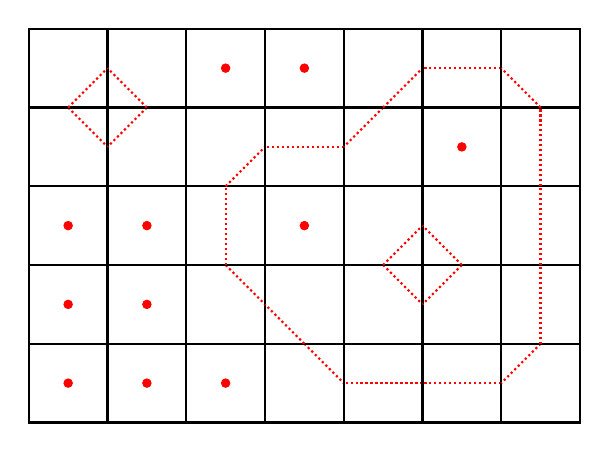
\begin{tikzpicture}
        % row1
        \cellopen{0}{0}{1}{1}
        \cellopen{1}{0}{2}{1}
        \cellopen{2}{0}{3}{1}
        \cellC{3}{0}{4}{1}
        \cellE{4}{0}{5}{1}
        \cellE{5}{0}{6}{1}
        \cellD{6}{0}{7}{1}
        % row2
        \cellopen{0}{1}{1}{2}
        \cellopen{1}{1}{2}{2}
        \cellC{2}{1}{3}{2}
        \cellA{3}{1}{4}{2}
        \cellC{4}{1}{5}{2}
        \cellD{5}{1}{6}{2}
        \cellF{6}{1}{7}{2}
        % row3
        \cellopen{0}{2}{1}{3}
        \cellopen{1}{2}{2}{3}
        \cellF{2}{2}{3}{3}
        \cellopen{3}{2}{4}{3}
        \cellB{4}{2}{5}{3}
        \cellA{5}{2}{6}{3}
        \cellF{6}{2}{7}{3}
        % row4
        \cellC{0}{3}{1}{4}
        \cellD{1}{3}{2}{4}
        \cellB{2}{3}{3}{4}
        \cellE{3}{3}{4}{4}
        \cellD{4}{3}{5}{4}
        \cellopen{5}{3}{6}{4}
        \cellF{6}{3}{7}{4}
        % row5
        \cellB{0}{4}{1}{5}
        \cellA{1}{4}{2}{5}
        \cellopen{2}{4}{3}{5}
        \cellopen{3}{4}{4}{5}
        \cellB{4}{4}{5}{5}
        \cellE{5}{4}{6}{5}
        \cellA{6}{4}{7}{5}

    \end{tikzpicture}
\end{center}
\caption{Mosaic Diagram of Binary Lattice in Figure \ref{fig:example of f mapping}}
\label{fig: mosaic diagram}
\end{figure}

One would hope that the function $u$ could be used to compute $|\mathbb{S}^{(m,n)}|$ in some way. However for the $(m,n)$ binary lattice $\ell^*$, we have

$$u(\ell^*) = 7^{mn} = |\mathbb{M}^{(m,n)}| > |\mathbb{S}^{(m,n)}|.$$

Clearly, this approach overcounts $|\mathbb{S}^{(m,n)}|$. We can examine this phenomena more closely by first definining $g$.

\begin{definition}
    $g: \mathbb{F}^{(m,n)} \to \mathbb{M}^{(m,n)}$ takes a framed binary lattice that does not contain the cells $\begin{smallmatrix} 0 & 1 \\ 1 & 0 \end{smallmatrix}$ or $\begin{smallmatrix} 1 & 0 \\ 0 & 1 \end{smallmatrix}$, and constructs a mosaic by replacing all $\begin{smallmatrix} 0 & 0 \\ 0 & 0 \end{smallmatrix}$ and $\begin{smallmatrix} 1 & 1 \\ 1 & 1 \end{smallmatrix}$ cells with $T_{0}$, and replacing all other cells with the unique tile that maps to that cell under $f$. 
\end{definition}

Notice that for some binary lattice $\ell$, $g(\ell)$ is not necessarily equal to $f^{-1}(\ell)$, as $g$ only returns polygon mosaics and not messy polygon mosaics. We can now examine the overcounting more closely.

\begin{exmp}

Consider the following binary lattices and mosaics for $(m,n)=(4,2)$. 

\begin{center}
    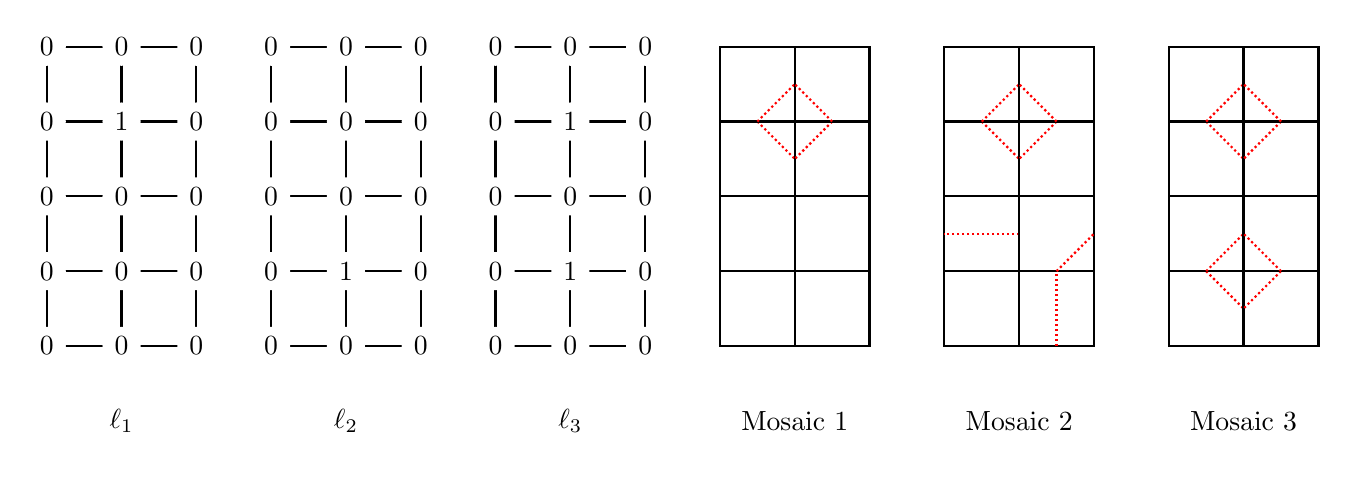
\begin{tikzpicture}[scale=0.95]

        % row1
        \cell{-3}{0}{-2}{1}
        \cell{-3}{1}{-2}{2}
        \cell{-3}{2}{-2}{3}
        \cell{-3}{3}{-2}{4}
        \cell{-2}{0}{-1}{1}
        \cell{-2}{1}{-1}{2}
        \cell{-2}{2}{-1}{3}
        \cell{-2}{3}{-1}{4}

        \( \lablnode{-2}{-1}{$\ell_{1}$} \)

        \( \lablvertex{-3}{0}{$0$} \)
        \( \lablvertex{-2}{0}{$0$} \)
        \( \lablvertex{-1}{0}{$0$} \)

        \( \lablvertex{-3}{1}{$0$} \)
        \( \lablvertex{-2}{1}{$0$} \)
        \( \lablvertex{-1}{1}{$0$} \)

        \( \lablvertex{-3}{2}{$0$} \)
        \( \lablvertex{-2}{2}{$0$} \)
        \( \lablvertex{-1}{2}{$0$} \)

        \( \lablvertex{-3}{3}{$0$} \)
        \( \lablvertex{-2}{3}{$1$} \)
        \( \lablvertex{-1}{3}{$0$} \)

        \( \lablvertex{-3}{4}{$0$} \)
        \( \lablvertex{-2}{4}{$0$} \)
        \( \lablvertex{-1}{4}{$0$} \)

        % row1
        \cell{0}{0}{1}{1}
        \cell{0}{1}{1}{2}
        \cell{0}{2}{1}{3}
        \cell{0}{3}{1}{4}
        \cell{1}{0}{2}{1}
        \cell{1}{1}{2}{2}
        \cell{1}{2}{2}{3}
        \cell{1}{3}{2}{4}

        \( \lablnode{1}{-1}{$\ell_{2}$} \)
        
        \( \lablvertex{0}{0}{$0$} \)
        \( \lablvertex{1}{0}{$0$} \)
        \( \lablvertex{2}{0}{$0$} \)

        \( \lablvertex{0}{1}{$0$} \)
        \( \lablvertex{1}{1}{$1$} \)
        \( \lablvertex{2}{1}{$0$} \)

        \( \lablvertex{0}{2}{$0$} \)
        \( \lablvertex{1}{2}{$0$} \)
        \( \lablvertex{2}{2}{$0$} \)

        \( \lablvertex{0}{3}{$0$} \)
        \( \lablvertex{1}{3}{$0$} \)
        \( \lablvertex{2}{3}{$0$} \)

        \( \lablvertex{0}{4}{$0$} \)
        \( \lablvertex{1}{4}{$0$} \)
        \( \lablvertex{2}{4}{$0$} \)

        % row1
        \cell{3}{0}{4}{1}
        \cell{3}{1}{4}{2}
        \cell{3}{2}{4}{3}
        \cell{3}{3}{4}{4}
        \cell{4}{0}{5}{1}
        \cell{4}{1}{5}{2}
        \cell{4}{2}{5}{3}
        \cell{4}{3}{5}{4}

        \( \lablnode{4}{-1}{$\ell_{3}$} \)

        \( \lablvertex{3}{0}{$0$} \)
        \( \lablvertex{4}{0}{$0$} \)
        \( \lablvertex{5}{0}{$0$} \)

        \( \lablvertex{3}{1}{$0$} \)
        \( \lablvertex{4}{1}{$1$} \)
        \( \lablvertex{5}{1}{$0$} \)

        \( \lablvertex{3}{2}{$0$} \)
        \( \lablvertex{4}{2}{$0$} \)
        \( \lablvertex{5}{2}{$0$} \)

        \( \lablvertex{3}{3}{$0$} \)
        \( \lablvertex{4}{3}{$1$} \)
        \( \lablvertex{5}{3}{$0$} \)

        \( \lablvertex{3}{4}{$0$} \)
        \( \lablvertex{4}{4}{$0$} \)
        \( \lablvertex{5}{4}{$0$} \)

        \cell{6}{0}{7}{1}
        \cell{7}{0}{8}{1}

        \cell{6}{1}{7}{2}
        \cell{7}{1}{8}{2}

        \cellC{6}{2}{7}{3}
        \cellD{7}{2}{8}{3}    

        \cellB{6}{3}{7}{4}
        \cellA{7}{3}{8}{4}    

        \( \lablnode{7}{-1}{Mosaic $1$} \)

        \cell{9}{0}{10}{1}
        \cellF{10}{0}{11}{1}

        \cellE{9}{1}{10}{2}
        \cellB{10}{1}{11}{2}

        \cellC{9}{2}{10}{3}
        \cellD{10}{2}{11}{3}    

        \cellB{9}{3}{10}{4}
        \cellA{10}{3}{11}{4}    

        \( \lablnode{10}{-1}{Mosaic $2$} \)

        \cellC{12}{0}{13}{1}
        \cellD{13}{0}{14}{1}

        \cellB{12}{1}{13}{2}
        \cellA{13}{1}{14}{2}

        \cellC{12}{2}{13}{3}
        \cellD{13}{2}{14}{3}    

        \cellB{12}{3}{13}{4}
        \cellA{13}{3}{14}{4}    

        \( \lablnode{13}{-1}{Mosaic $3$} \)

    \end{tikzpicture}
\end{center}

We have $u(\ell_1) = 7^4, u(\ell_2) = 7^4,$ and $u(\ell_3) = 1$. We also have $f(\text{Mosaic } 3) = \ell_3$. Each cell in the bottom two rows of $\ell_1$ map to $7$ possible tiles. However, $1$ of the $7^4$ combinations forms a new polygon in these bottom two rows. This is also true for the top two rows of $\ell_2$. Therefore, $u(\ell_1)$, $u(\ell_2)$, and $u(\ell_3)$ all count Mosaic $3$.

\label{exmp:U doesnt work}
\end{exmp}

Example \ref{exmp:U doesnt work} leads us to conclude the following.

\begin{prop}
For a framed binary lattice $\ell$ that does not contain the cells $\begin{smallmatrix} 0 & 1 \\ 1 & 0 \end{smallmatrix}$ or $\begin{smallmatrix} 1 & 0 \\ 0 & 1 \end{smallmatrix}$, $u(\ell)$ counts the number of mosaics that have at least the polygons in $g(\ell)$.
\label{prop: u counts atleast g l}
\end{prop}

\begin{proof}
Choose an framed binary lattice $\ell$ that does not contain the cells $\begin{smallmatrix} 0 & 1 \\ 1 & 0 \end{smallmatrix}$ or $\begin{smallmatrix} 1 & 0 \\ 0 & 1 \end{smallmatrix}$. By the definition of $g$, the function $u(\ell)$ counts the number of mosaics that have exactly the polygons in $g(\ell)$. Additionally, as $u$ counts each possible combination of tiles for $\begin{smallmatrix} 0 & 0 \\ 0 & 0 \end{smallmatrix}$ and $\begin{smallmatrix} 1 & 1 \\ 1 & 1 \end{smallmatrix}$ cells, this includes all polygons that do not conflict with the polygons in $g(\ell)$.
\end{proof}

Surprisingly, this overcounting phenomena can be remedied by a small modificiation to $u$, which we call $v$.

\begin{definition}
Let $v: \mathbb{L}^{(m,n)} \to \mathbb{Z}$ map a binary lattice $\ell$ to the product over all cells in $\ell$ with each term being $$\begin{cases}
    7 & \text{for cells } \begin{smallmatrix} 0 & 0 \\ 0 & 0 \end{smallmatrix}, \begin{smallmatrix} 1 & 1 \\ 1 & 1 \end{smallmatrix}\\
    0 & \text{for cells } \begin{smallmatrix} 0 & 1 \\ 1 & 0 \end{smallmatrix}, \begin{smallmatrix} 1 & 0 \\ 0 & 1 \end{smallmatrix}\\
    -1 & \text{for cells } \begin{smallmatrix} 0 & 0 \\ 1 & 0 \end{smallmatrix}, \begin{smallmatrix} 1 & 0 \\ 1 & 1 \end{smallmatrix}\\
    1 & \text{otherwise}
\end{cases}$$

and the empty product being $1$.
\label{def: def of v}
\end{definition}

\begin{exmp}
\label{exmp: v on a ell}
If we let $\ell$ be the framed binary lattice on the right of Figure \ref{fig:example of f mapping}, we have $v(\ell) = -7^{11}$.
\end{exmp}

We will first show that $v(\ell)$, which is computed ``cell-by-cell'' from $\ell$, recovers global information about the number of polygons in $g(\ell)$ if $\ell$ is framed.

\begin{definition}
For a framed binary lattice $\ell$, let $P(\ell)$ to be the number of polygons in the polygon mosaic $g(\ell)$.
\end{definition}

\begin{prop} 
If $\ell$ is a framed binary lattice that does not contain the cells $\begin{smallmatrix} 0 & 1 \\ 1 & 0 \end{smallmatrix}$ or $\begin{smallmatrix} 1 & 0 \\ 0 & 1 \end{smallmatrix}$, then 
\begin{equation}
\text{sign}(v(\ell)) = (-1)^{P(\ell)}.
\label{eq: sign prop}
\end{equation}
\label{prop: sign of v}
\end{prop}

\begin{proof}

For this proof, we use LHS and RHS to abbreviate the left and right hand side of Equation \ref{eq: sign prop}. We prove the result by induction. For the base case, construct the $(1,n)$ framed binary lattice $\ell$ for some $n \geq 1$. As there are no cells in $\ell$, from the definition of $v$ the LHS is $v(\ell)=1$. As there no polygons in $g(\ell)$, we have the RHS is $1$.

For the induction step, fix an $(m,n)$ framed binary strip $\ell$ for $m \geq 1$. Then consider an $(m+1,n)$ framed binary strip $\ell'$ that shares the top $m-1$ rows of vertices with $\ell$ and an arbitrarily-labeled $m$-th row, such that there are no $\begin{smallmatrix} 0 & 1 \\ 1 & 0 \end{smallmatrix}$ or $\begin{smallmatrix} 1 & 0 \\ 0 & 1 \end{smallmatrix}$ cells. We show that we can construct $\ell'$ from $\ell$ with a procedure that preserves Equation \ref{eq: sign prop} with each intermediate step.

\noindent\textbf{Procedure:} \\
\indent \textbf{Step a.} Add a bottom row to $\ell$ of $n+1$ vertices all labeled $0$. This results in a new $(m+1,n)$ framed binary lattice we denote $\ell_a$. \\
\indent \textbf{Step b.} Scanning rows $m-1$ and $m$ of $\ell'$ left to right, if there exists a column of the form $\begin{smallmatrix} 1 \\ 1 \end{smallmatrix}$, change the associated $\begin{smallmatrix} 1 \\ 0 \end{smallmatrix}$ column in $\ell_a$ to $\begin{smallmatrix} 1 \\ 1 \end{smallmatrix}$. Completing this scan results in a new framed binary lattice denoted $\ell_b$.\\
\indent \textbf{Step c.} Scanning rows $m-1$ and $m$ of $\ell'$ left to right, if there exists a column of the form $\begin{smallmatrix} 0 \\ 1 \end{smallmatrix}$, change the associated $\begin{smallmatrix} 0 \\ 0 \end{smallmatrix}$ column in $\ell_b$ to $\begin{smallmatrix} 0 \\ 1 \end{smallmatrix}$. Completing this scan results in the framed binary lattice $\ell'$.\\

For step a, only $\begin{smallmatrix} 0 & 0 \\ 0 & 0 \end{smallmatrix}$ cells are added. As $\text{sign}\left(v\left(\begin{smallmatrix} 0 & 0 \\ 0 & 0 \end{smallmatrix}\right)\right) = 1$, the LHS is unchanged. For the RHS, no new edge-connected regions are created, no new polygons are created in $g(\ell_a)$ so Equation \ref{eq: sign prop} is preserved by step a.

For steps b and c, we encounter two distinct cases which we diagram in Figure \ref{fig: step diagrams}. These diagrams have $a,b,c,d \in [0, 1]$, and use the \# symbol to indicate the vertex being changed from a $0$ to a $1$.

\begin{figure}[h!]
\centering
\begin{subfigure}[t]{0.4\textwidth}
\begin{center}
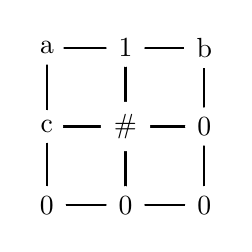
\begin{tikzpicture}
% row 1 of cells
\cell{0}{0}{1}{1}
\cell{1}{0}{2}{1}
% row 2 of cells
\cell{0}{-1}{1}{0}
\cell{1}{-1}{2}{0}
% row 1 labels
\( \lablvertex{0}{0}{c} \)
\( \lablvertex{1}{0}{\#} \)
\( \lablvertex{2}{0}{$0$} \)
% row 2 labels
\( \lablvertex{0}{1}{a} \)
\( \lablvertex{1}{1}{$1$} \)
\( \lablvertex{2}{1}{b} \)
% row 3 labels
\( \lablvertex{0}{-1}{$0$} \)
\( \lablvertex{1}{-1}{$0$} \)
\( \lablvertex{2}{-1}{$0$} \)
\end{tikzpicture}
\end{center}
\caption{Step b. Diagram}
\label{subfig: step b diagram}
\end{subfigure}
~
\begin{subfigure}[t]{0.4\textwidth}
\begin{center}
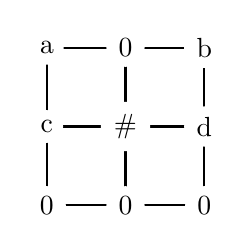
\begin{tikzpicture}
% row 1 of cells
\cell{0}{0}{1}{1}
\cell{1}{0}{2}{1}
% row 1 of cells
\cell{0}{-1}{1}{0}
\cell{1}{-1}{2}{0}
% row 1 labels
\( \lablvertex{0}{0}{c} \)
\( \lablvertex{1}{0}{\#} \)
\( \lablvertex{2}{0}{d} \)
% row 2 labels
\( \lablvertex{0}{1}{a} \)
\( \lablvertex{1}{1}{$0$} \)
\( \lablvertex{2}{1}{b} \)
% row -1 labels
\( \lablvertex{0}{-1}{$0$} \)
\( \lablvertex{1}{-1}{$0$} \)
\( \lablvertex{2}{-1}{$0$} \)
\end{tikzpicture}
\end{center}
\caption{Step c. Diagram}
\label{subfig: step c diagram}
\end{subfigure}
\caption{Step Diagrams}
\label{fig: step diagrams}
\end{figure}

For step b, Figure  \ref{subfig: step b diagram} depicts all possible cases one can encounter scanning left to right on $\ell_a$. Note that the vertex right of the \# symbol must be $0$, as the procedure moving left to right on $\ell_a$ gives that this vertex must be $0$.

Notice that no assignment of $a$, $b$, and $c$ can create cells $\begin{smallmatrix} 0 & 0 \\ 1 & 0 \end{smallmatrix}$ or $\begin{smallmatrix} 1 & 0 \\ 1 & 1 \end{smallmatrix}$. Additionally, it cannot be the case that $a=0$ and $c=1$, as that would imply that $\ell'$ contains the cell $\begin{smallmatrix} 0 & 1 \\ 1 & 0 \end{smallmatrix}$. Therefore we have $\text{sign}(v(\ell_b)) = \text{sign}(v(\ell_a))$, so the LHS is preserved. Also note that because a polygon in $g(\ell)$ is an edge-connected set of vertices with the same label (not including the boundary $0$'s), that for all assignments of $a,b,c$, step b only involves one edge-connected set of vertices. Therefore, we have $P(\ell_a) = P(\ell_b)$, and so the RHS is preserved.

For step c, Figure \ref{subfig: step c diagram} depicts all possible cases one can encounter scanning left to right on $\ell_b$. It cannot be the case that $a=1$ and $c=0$, as this would imply $\ell'$ contains $\begin{smallmatrix} 1 & 0 \\ 0 & 1 \end{smallmatrix}$. Similarly, it cannot be the cases that $b=1$ and $d=0$, as this would imply $\ell_b$ contains $\begin{smallmatrix} 0 & 1 \\ 1 & 0 \end{smallmatrix}$. Additionally, it cannot be the case that $b=0$ and $d=1$, as the procedure moves left-to-right. This results in the following $6$ cases, which we show each preserve Equation \ref{eq: sign prop}.

\begin{figure}[h!]
\centering
\begin{subfigure}[t]{0.2\textwidth}
\begin{center}
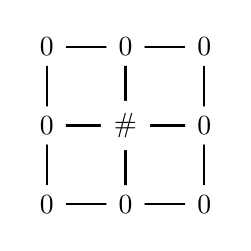
\begin{tikzpicture}
% row 1 of cells
\cell{0}{0}{1}{1}
\cell{1}{0}{2}{1}
\cell{0}{-1}{1}{0}
\cell{1}{-1}{2}{0}
% row 1 labels
\( \lablvertex{0}{0}{$0$} \)
\( \lablvertex{1}{0}{\#} \)
\( \lablvertex{2}{0}{$0$} \)
% row 2 labels
\( \lablvertex{0}{1}{$0$} \)
\( \lablvertex{1}{1}{$0$} \)
\( \lablvertex{2}{1}{$0$} \)
% row -1 labels
\( \lablvertex{0}{-1}{$0$} \)
\( \lablvertex{1}{-1}{$0$} \)
\( \lablvertex{2}{-1}{$0$} \)
\end{tikzpicture}
\end{center}
\caption{}
\label{subfig: bit flip case 1}
\end{subfigure}
~
\begin{subfigure}[t]{0.2\textwidth}
\begin{center}
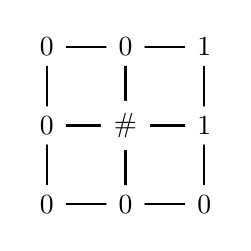
\begin{tikzpicture}
% row 1 of cells
\cell{0}{0}{1}{1}
\cell{1}{0}{2}{1}
\cell{0}{-1}{1}{0}
\cell{1}{-1}{2}{0}
% row 1 labels
\( \lablvertex{0}{0}{$0$} \)
\( \lablvertex{1}{0}{\#} \)
\( \lablvertex{2}{0}{$1$} \)
% row 2 labels
\( \lablvertex{0}{1}{$0$} \)
\( \lablvertex{1}{1}{$0$} \)
\( \lablvertex{2}{1}{$1$} \)
% row -1 labels
\( \lablvertex{0}{-1}{$0$} \)
\( \lablvertex{1}{-1}{$0$} \)
\( \lablvertex{2}{-1}{$0$} \)
\end{tikzpicture}
\end{center}
\caption{}
\label{subfig: bit flip case 2}
\end{subfigure}
~
\begin{subfigure}[t]{0.2\textwidth}
\begin{center}
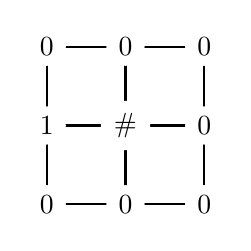
\begin{tikzpicture}
% row 1 of cells
\cell{0}{0}{1}{1}
\cell{1}{0}{2}{1}
\cell{0}{-1}{1}{0}
\cell{1}{-1}{2}{0}
% row 1 labels
\( \lablvertex{0}{0}{$1$} \)
\( \lablvertex{1}{0}{\#} \)
\( \lablvertex{2}{0}{$0$} \)
% row 2 labels
\( \lablvertex{0}{1}{$0$} \)
\( \lablvertex{1}{1}{$0$} \)
\( \lablvertex{2}{1}{$0$} \)
% row -1 labels
\( \lablvertex{0}{-1}{$0$} \)
\( \lablvertex{1}{-1}{$0$} \)
\( \lablvertex{2}{-1}{$0$} \)
\end{tikzpicture}
\end{center}
\caption{}
\label{subfig: bit flip case 3}
\end{subfigure}

% \hfill

\begin{subfigure}[t]{0.2\textwidth}
\begin{center}
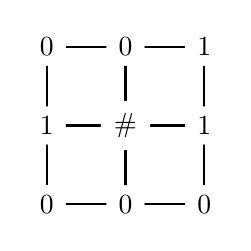
\begin{tikzpicture}
% row 1 of cells
\cell{0}{0}{1}{1}
\cell{1}{0}{2}{1}
\cell{0}{-1}{1}{0}
\cell{1}{-1}{2}{0}
% row 1 labels
\( \lablvertex{0}{0}{$1$} \)
\( \lablvertex{1}{0}{\#} \)
\( \lablvertex{2}{0}{$1$} \)
% row 2 labels
\( \lablvertex{0}{1}{$0$} \)
\( \lablvertex{1}{1}{$0$} \)
\( \lablvertex{2}{1}{$1$} \)
% row -1 labels
\( \lablvertex{0}{-1}{$0$} \)
\( \lablvertex{1}{-1}{$0$} \)
\( \lablvertex{2}{-1}{$0$} \)
\end{tikzpicture}
\end{center}
\caption{}
\label{subfig: bit flip case 4}
\end{subfigure}
~
\begin{subfigure}[t]{0.2\textwidth}
\begin{center}
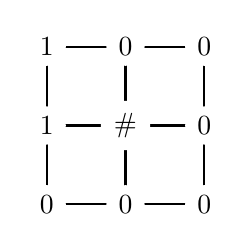
\begin{tikzpicture}
% row 1 of cells
\cell{0}{0}{1}{1}
\cell{1}{0}{2}{1}
\cell{0}{-1}{1}{0}
\cell{1}{-1}{2}{0}
% row 1 labels
\( \lablvertex{0}{0}{$1$} \)
\( \lablvertex{1}{0}{\#} \)
\( \lablvertex{2}{0}{$0$} \)
% row 2 labels
\( \lablvertex{0}{1}{$1$} \)
\( \lablvertex{1}{1}{$0$} \)
\( \lablvertex{2}{1}{$0$} \)
% row -1 labels
\( \lablvertex{0}{-1}{$0$} \)
\( \lablvertex{1}{-1}{$0$} \)
\( \lablvertex{2}{-1}{$0$} \)
\end{tikzpicture}
\end{center}
\caption{}
\label{subfig: bit flip case 5}
\end{subfigure}
~
\begin{subfigure}[t]{0.2\textwidth}
\begin{center}
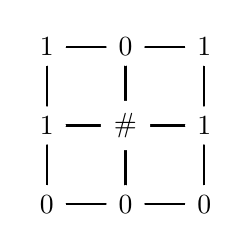
\begin{tikzpicture}
% row 1 of cells
\cell{0}{0}{1}{1}
\cell{1}{0}{2}{1}
\cell{0}{-1}{1}{0}
\cell{1}{-1}{2}{0}
% row 1 labels
\( \lablvertex{0}{0}{$1$} \)
\( \lablvertex{1}{0}{\#} \)
\( \lablvertex{2}{0}{$1$} \)
% row 2 labels
\( \lablvertex{0}{1}{$1$} \)
\( \lablvertex{1}{1}{$0$} \)
\( \lablvertex{2}{1}{$1$} \)
% row -1 labels
\( \lablvertex{0}{-1}{$0$} \)
\( \lablvertex{1}{-1}{$0$} \)
\( \lablvertex{2}{-1}{$0$} \)
\end{tikzpicture}
\end{center}
\caption{}
\label{subfig: bit flip case 6}
\end{subfigure}
\caption{Step c. Cases}
\label{fig: }
\end{figure}

In Case \ref{subfig: bit flip case 1}, the flip add one $\begin{smallmatrix} 0 & 0 \\ 1 & 0 \end{smallmatrix}$ cell, so the sign of the LHS changes. As the flip creates a new edge-connected region, a new polygon is created, and so the sign of the RHS changes. 

In Case \ref{subfig: bit flip case 2}, the flip does not add a $\begin{smallmatrix} 0 & 0 \\ 1 & 0 \end{smallmatrix}$ cell or $\begin{smallmatrix} 1 & 0 \\ 1 & 1 \end{smallmatrix}$ cell, so the sign of the LHS stays the same. As the flip does not create a new edge-connected region, the RHS stays the same.

In Case \ref{subfig: bit flip case 3}, the flip removes and adds a $\begin{smallmatrix} 0 & 0 \\ 1 & 0 \end{smallmatrix}$ cell, so the sign of the LHS stays the same. As the flip does not create a new edge-connected region, the RHS stays the same.

In Case \ref{subfig: bit flip case 4}, the flip removes a $\begin{smallmatrix} 0 & 0 \\ 1 & 0 \end{smallmatrix}$ cell, so the sign of the LHS changes. Before the flip, either the two edge-connected regions of $1$'s are distinct in the full framed binary lattice, or they are joined. After the flip, if the regions were distinct, they are now joined, and so $1$ polygon is removed. If the regions were joined, a new edge-connected region of $0$'s (that is not connected to the boundary) is created, and so $1$ polygon is created. Either way, the RHS changes.

In Case \ref{subfig: bit flip case 5}, the flip adds both a $\begin{smallmatrix} 0 & 0 \\ 1 & 0 \end{smallmatrix}$ cell and a $\begin{smallmatrix} 1 & 0 \\ 1 & 1 \end{smallmatrix}$ cell, so the sign of the LHS stays the same. As the flip does not create a new edge-connected region, the RHS stays the same.

In Case \ref{subfig: bit flip case 6}, the flip adds $\begin{smallmatrix} 1 & 0 \\ 1 & 1 \end{smallmatrix}$, so the sign of the LHS changes. The same logic from Case \ref{subfig: bit flip case 4} applies, as the flip either removes or adds a polygon, so the RHS changes.

As all cases preserve Equation \ref{eq: sign prop}, the $(m+1, n)$ framed binary lattice $\ell'$ also follows Equation \ref{eq: sign prop}.
\end{proof}

We point out here that the function $v$ if defined for all binary lattices, while Proposition \ref{prop: sign of v} only holds for framed binary lattices that do not contain cells $\begin{smallmatrix} 0 & 1 \\ 1 & 0 \end{smallmatrix}$ or $\begin{smallmatrix} 1 & 0 \\ 0 & 1 \end{smallmatrix}$.

\begin{prop}
The number of $(m,n)$ mosaics that do not contain a polygon has
$$\left|\mathbb{S}^{(m,n)}\right| = \sum_{\ell \in \mathbb{F}^{(m,n)}}v(\ell).$$
\label{prop: sum of vs}
\end{prop}

\begin{proof}
Choose a mosaic $\mathcal{M}$ that has $P(\ell')$ polygons, where $\ell' = f(\mathcal{M})$. We begin by determining how many times $\mathcal{M}$ is counted in the related sum

$$\sum_{\ell \in \mathbb{F}^{(m,n)}}u(\ell).$$

We point out here that as $u(\begin{smallmatrix} 0 & 1 \\ 1 & 0 \end{smallmatrix}) = u(\begin{smallmatrix} 1 & 0 \\ 0 & 1 \end{smallmatrix}) = v(\begin{smallmatrix} 0 & 1 \\ 1 & 0 \end{smallmatrix}) = v(\begin{smallmatrix} 1 & 0 \\ 0 & 1 \end{smallmatrix}) = 0$, framed binary lattices with these cells don't contribute to either summation, and so can be ignored for the remainder of this argument.

Proposition \ref{prop: u counts atleast g l} shows that the function $u(\ell)$ counts the mosaics with at least the polygons in $g(\ell)$. Consequently, for a framed binary lattice $\ell$, $u(\ell)$ counts $\mathcal{M}$ if the polygons in $g(\ell)$ are a subset of the polygons in $\mathcal{M}$. Therefore, as the number of ways to choose a size $p$ subset of $P(\ell)$ polygons is $\binom{P(\ell)}{p}$, $\mathcal{M}$ is counted $\sum_{p=0}^{P(\ell)}\binom{P(\ell)}{p}$ times. This then gives

$$\sum_{\ell \in \mathbb{F}^{(m,n)}}u(\ell) = \sum_{\mathcal{M} \in \mathbb{M}^{(m,n)}}\sum_{p=0}^{P(f(\mathcal{M}))}\binom{P(f(\mathcal{M}))}{p}.$$

Following the same logic for $\sum_{\ell \in \mathbb{F}^{(m,n)}} v(\ell)$, Proposition \ref{prop: sign of v} gives that size $p$ subsets where $p$ is odd are subtracted, which gives

$$\sum_{\ell \in \mathbb{F}^{(m,n)}} v(\ell) = \sum_{\mathcal{M} \in \mathbb{M}^{(m,n)}}\sum_{p=0}^{P(f(\mathcal{M}))}(-1)^{p}\binom{P(f(\mathcal{M}))}{p}.$$

Finally, by the binomial theorem, for $P(\ell) > 0$ we have

$$\sum_{p=0}^{P(\ell)}(-1)^{p}\binom{P(\ell)}{p} = 0,$$

and as the only binary lattice with $P(\ell) = 0$ is $\ell^*$, we have

$$\sum_{\ell \in \mathbb{F}^{(m,n)}} v(\ell) = \sum_{\{\mathcal{M} \in \mathbb{M}^{(m,n)} | P(f(\mathcal{M})) = 0\}}\binom{0}{0} = |f^{-1}(\ell^*)| = |\mathbb{S}^{(m,n)}|.$$

\end{proof}

As in Theorem \ref{thm:Oh2014} from \cite{Oh2014}, we can compute $\sum_{\ell \in \mathbb{F}^{(m,n)}}v(\ell)$ efficiently using the state matrix recursion method.

\section{Proof of Theorem \ref{thm: messy mosaics}}

We begin by defining the state matrices.

\begin{definition}

Let $A_k, B_k, C_k, D_k$ be $2^{k-1} \times 2^{k-1}$ matrices with integer entries, where $A_{1}=\begin{pmatrix}v(\begin{smallmatrix} 0 & 0 \\ 0 & 0 \end{smallmatrix})\end{pmatrix}, B_{1}=\begin{pmatrix}v(\begin{smallmatrix} 0 & 0 \\ 1 & 0 \end{smallmatrix})\end{pmatrix}, C_{1}=\begin{pmatrix}v(\begin{smallmatrix} 1 & 0 \\ 0 & 0 \end{smallmatrix})\end{pmatrix}, D_{1}=\begin{pmatrix}v(\begin{smallmatrix} 1 & 0 \\ 1 & 0 \end{smallmatrix})\end{pmatrix}$, and for integers $k \geq 1$,

\begin{eqnarray*}
A_{k+1} = \begin{pmatrix} v(\begin{smallmatrix} 0 & 0 \\ 0 & 0 \end{smallmatrix})A_{k} & v(\begin{smallmatrix} 0 & 0 \\ 0 & 1 \end{smallmatrix})B_{k} \\ v(\begin{smallmatrix} 0 & 1 \\ 0 & 0 \end{smallmatrix})C_{k} & v(\begin{smallmatrix} 0 & 1 \\ 0 & 1 \end{smallmatrix})D_{k} \end{pmatrix} & B_{k+1} = \begin{pmatrix} v(\begin{smallmatrix} 0 & 0 \\ 1 & 0 \end{smallmatrix})A_{k} & v(\begin{smallmatrix} 0 & 0 \\ 1 & 1 \end{smallmatrix})B_{k} \\ v(\begin{smallmatrix} 0 & 1 \\ 1 & 0 \end{smallmatrix})C_{k} & v(\begin{smallmatrix} 0 & 1 \\ 1 & 1 \end{smallmatrix})D_{k} \end{pmatrix} \\
C_{k+1} = \begin{pmatrix} v(\begin{smallmatrix} 1 & 0 \\ 0 & 0 \end{smallmatrix})A_{k} & v(\begin{smallmatrix} 1 & 0 \\ 0 & 1 \end{smallmatrix})B_{k} \\ v(\begin{smallmatrix} 1 & 1 \\ 0 & 0 \end{smallmatrix})C_{k} & v(\begin{smallmatrix} 1 & 1 \\ 0 & 1 \end{smallmatrix})D_{k} \end{pmatrix} & D_{k+1} = \begin{pmatrix} v(\begin{smallmatrix} 1 & 0 \\ 1 & 0 \end{smallmatrix})A_{k} & v(\begin{smallmatrix} 1 & 0 \\ 1 & 1 \end{smallmatrix})B_{k} \\ v(\begin{smallmatrix} 1 & 1 \\ 1 & 0 \end{smallmatrix})C_{k} & v(\begin{smallmatrix} 1 & 1 \\ 1 & 1 \end{smallmatrix})D_{k} \end{pmatrix}.
\end{eqnarray*}
\end{definition}

\begin{definition}
Let the $n$ digit binary representation of the number $k$ be written as $\beta_n(k)$. If $k$ is $0$, $\beta_k(n)$ returns the empty string.
\end{definition}

\begin{prop}
The $(i,j)$-th entry of $A_{n}$ is $v(\ell)$, where $\ell$ is the $(1, n)$ binary lattice where the top row of vertices has labels $0\beta_{n-1}(i)0$ and the bottom row of vertices has labels $0\beta_{n-1}(j)0$, both read left to right. Furthermore, the same statement is true for $B_{n}$ with top row $1\beta_{n-1}(i)0$ and bottom row $0\beta_{n-1}(j)0$, for $C_{n}$ with top row $0\beta_{n-1}(i)0$ and bottom row $1\beta_{n-1}(j)0$, and for $D_{n}$ with top row $1\beta_{n-1}(i)0$ and bottom row $1\beta_{n-1}(j)0$.
\label{prop: one by n state matrix}
\end{prop}

\begin{proof}
We prove by induction. For $n=1$, the definition of the state matrices gives $A_1$ is $v(\ell)$ where $\ell$ is the $(1,1)$ binary lattice with top row $0\beta_0(0)0=00$ and bottom row $0\beta_0(0)0=00$, as $\beta_0(0)$ is the empty string. The same is true for $B_1$ with top row $0\beta_0(0)0=10$ and bottom row $1\beta_0(0)0=00$, for $C_1$ with top row $1\beta_0(0)0=00$ and bottom row $0\beta_0(0)0=10$, and for $D_1$ with top row $1\beta_0(0)0=10$ and bottom row $1\beta_0(0)0=10$.

We next assume matrices $A_n, B_n, C_n$, and $D_n$ follow their associated statements in Proposition \ref{prop: one by n state matrix}. Therefore, the entry $(i,j)$ in, say, $B_n$ is $v(\ell)$ where $\ell$ is the binary lattice with top row $0\beta_{n-1}(i)0$ and bottom row $1\beta_{n-1}(j)0$. The argument is analagous for any choice of $A_n, B_n, C_n, D_n$. For $n > 1$ we can depict the $(1,n)$ binary lattice using similar notation to cells, namely

$$v(\ell) = v\left(\begin{smallmatrix} 0 & \beta_{n-1}(i) & 0 \\ 1 & \beta_{n-1}(j) & 0 \end{smallmatrix}\right).$$

We show that $A_{n+1}$ also follows Proposition \ref{prop: one by n state matrix}. From the definition, we have

$$A_{n+1} = \begin{pmatrix} v(\begin{smallmatrix} 0 & 0 \\ 0 & 0 \end{smallmatrix})A_{n} & v(\begin{smallmatrix} 0 & 0 \\ 0 & 1 \end{smallmatrix})B_{n} \\ v(\begin{smallmatrix} 0 & 1 \\ 0 & 0 \end{smallmatrix})C_{n} & v(\begin{smallmatrix} 0 & 1 \\ 0 & 1 \end{smallmatrix})D_{n} \end{pmatrix}.$$

By construction, the $(i,j)$-th entry in $B_n$ is located in the $(i, j+2^{n-1})$-th entry of $A_{n+1}$, as each block matrix $A_n, B_n, C_n, D_n$ are $2^{n-1} \times 2^{n-1}$ matrices. Also by construction, the value in the $(i,j)$-th entry in $B_n$ which we call $v(\ell)$ is multiplied by $v(\begin{smallmatrix} 0 & 0 \\ 0 & 1 \end{smallmatrix})$. The definition of $v$ gives

$$v(\begin{smallmatrix} 0 & 0 \\ 0 & 1 \end{smallmatrix})v(\ell) = v\left(\begin{smallmatrix} 0 & 0 \\ 0 & 1 \end{smallmatrix}\right)v\left(\begin{smallmatrix} 0 & \beta_{n-1}(i) & 0 \\ 1 & \beta_{n-1}(j) & 0 \end{smallmatrix}\right) = v\left(\begin{smallmatrix} 0 & \beta_{n}(i) & 0 \\ 0 & \beta_{n}(j+2^{n-1}) & 0 \end{smallmatrix}\right),$$

Therefore, the $(i, j+2^{n-1})$-th entry of $A_{n+1}$ is $v(\ell)$ where $\ell$ is the $(1,n+1)$ binary lattice where the top row of vertices is $0\beta_{n}(i)0$ and the bottom row of vertices is $0\beta_{n}(j+2^{n-1})0$, which completes the induction step for $A_{n+1}$. Similar arguments hold for matrices $B_{n+1}$, $C_{n+1}$, $D_{n+1}$.

\end{proof}

\begin{prop}
The $(i,j)$-th entry of $A^{m}_{n}$ is $\sum_{\ell \in L}v(\ell)$, where $L$ is the set of $(m, n)$ binary lattices with the top row of vertices having labels $0\beta_{n-1}(i)0$ and the bottom row of vertices having labels $0\beta_{n-1}(j)0$, both read left to right.
\label{prop: m by n state matrix}
\end{prop}

\begin{proof}
We prove by induction. The base case $m=1$ is Proposition \ref{prop: one by n state matrix}, as the set $L$ only has the unique $(1,n)$ binary lattice.

We next assume that the $(i,j)$-th entry of $A^{m}_{n}$ satisfies the statement in Proposition \ref{prop: m by n state matrix}, and show the statement also holds for $A^{m+1}_{n}$. To begin, consider the product $A^{m}_{n} \cdot A_n$, and choose an integer $k \in [0, 2^{n-1}-1]$. From the induction hypothesis the value at the $(i,k)$-th entry of $A^{m}_{n}$ is $\sum_{\ell \in L}v(\ell)$, where $L$ is the set of $(m, n)$ binary lattices with the top row of vertices having labels $0\beta_{n-1}(i)0$ and the bottom row of vertices having labels $0\beta_{n-1}(k)0$. Similarly, the $(k, j)$-th entry of $A_n$ is the $(1,n)$ binary lattice $\begin{smallmatrix} 0 & \beta_{n-1}(k) & 0 \\ 0 & \beta_{n-1}(j) & 0 \end{smallmatrix}.$

Therefore, the dot product of the $i$-th row and the $j$-th column is $(i,j)$-th value of $A_n^{m+1}$, which is

$$\sum_{k=0}^{2^{n-1}-1}v\left(\begin{smallmatrix} 0 & \beta_{n-1}(i) & 0 \\ & \dots & \\ 0 & \beta_{n-1}(k) & 0 \end{smallmatrix}\right)v\left(\begin{smallmatrix} 0 & \beta_{n-1}(k) & 0 \\ 0 & \beta_{n-1}(j) & 0 \end{smallmatrix}\right) = v\left(\begin{smallmatrix} 0 & \beta_{n-1}(i) & 0 \\ & \dots & \\ 0 & \beta_{n-1}(j) & 0 \end{smallmatrix}\right),$$

which gives the desired result for $A_n^{m+1}$.
\end{proof}

\begin{prop}
The number of $(m,n)$ mosaics that do not contain a polygon is the $(0,0)$ entry of $A_{n}^m$.
\end{prop}

\begin{proof}
By Proposition \ref{prop: m by n state matrix}, the $(0,0)$ entry of $A^{m}_{n}$ is $\sum_{\ell \in L}v(\ell)$, where $L$ is the set of $(m, n)$ binary lattices with the top and bottom rows of vertices having labels $0\beta_{n-1}(0)0$. As $A$ has left-most and right-most columns all labeled $0$, all binary lattices counted at $(0,0)$ are framed, so $L = \mathbb{F}^{(m,n)}$. Substituting the values for $v$ from Definition \ref{def: def of v} gives the sum from Proposition \ref{prop: sum of vs}, which completes the proof.
\end{proof}

\section{Acknowledgements}

The authors would like to thank Richard Schank for his suggestions, including proposing the definition for $f$ and working to develop the state matrix recursion matrix solution.

% \newpage

\printbibliography

% \section{Appendix}

% \textbf{TODO}

\end{document}